\documentclass[aspectratio=169]{beamer}
\usetheme{Madrid}
\usecolortheme{default}

\usepackage{graphicx}
\usepackage{booktabs}
\usepackage{amsmath}
\usepackage{tikz}
\usetikzlibrary{positioning, shapes, arrows.meta}
\usepackage{pgfplots}
\pgfplotsset{compat=1.18}

\title[DRL Portfolio Optimization]{Deep Reinforcement Learning for Portfolio Optimization}
\subtitle{Achieving Superior Risk-Adjusted Returns with Options Overlay}
\author{CHONG Tin Tak}
\institute{HKUST - IEDA4000F}
\date{\today}

\begin{document}

% Title Slide
\begin{frame}
\titlepage
\end{frame}

% Table of Contents
\begin{frame}{Outline}
\tableofcontents
\end{frame}

% Section 1: Introduction
\section{Introduction}

\begin{frame}{The Portfolio Management Challenge}
\begin{columns}
\column{0.5\textwidth}
\textbf{Traditional Approaches:}
\begin{itemize}
    \item Manual decision-making
    \item Rule-based strategies
    \item Mean-variance optimisation
    \item Limited adaptability
\end{itemize}

\vspace{1em}
\textbf{Key Challenges:}
\begin{itemize}
    \item Market volatility
    \item Risk management
    \item Dynamic rebalancing
    \item Transaction costs
\end{itemize}

\column{0.4\textwidth}
\begin{left}
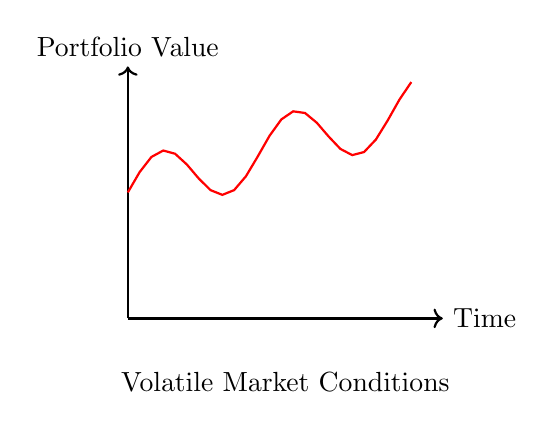
\begin{tikzpicture}[scale=0.8]
    \draw[thick,->] (0,0) -- (5,0) node[right] {Time};
    \draw[thick,->] (0,0) -- (0,4) node[above] {Portfolio Value};
    \draw[red, thick, domain=0:4.5] plot (\x, {2 + 0.3*\x + 0.5*sin(3*\x r)});
    \node at (2.5,-1) {Volatile Market Conditions};
\end{tikzpicture}
\end{left}
\end{columns}
\end{frame}

% Section 2: Motivation
\section{Motivation}

\begin{frame}{Why Reinforcement Learning?}
\begin{columns}
\column{0.6\textwidth}
\textbf{Limitations of Traditional ML:}
\begin{itemize}
    \item \textbf{Supervised Learning}: Requires labelled optimal actions (unknown in finance)
    \item \textbf{Regression Models}: Predict returns but don't make decisions
    \item \textbf{Classification}: Binary signals don't capture portfolio weights
    \item \textbf{Static Models}: Can't adapt to changing market regimes
\end{itemize}

\vspace{1em}
\textbf{RL Advantages:}
\begin{itemize}
    % \item[\checkmark] Learns from \textbf{experience}, not labels
    \item[\checkmark] \textbf{Sequential decision-making} over time
    \item[\checkmark] Balances \textbf{exploration vs. exploitation}
    \item[\checkmark] Optimizes \textbf{long-term rewards}, not just predictions
\end{itemize}

\column{0.2\textwidth}
\begin{center}
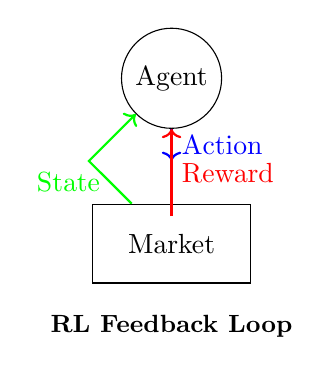
\begin{tikzpicture}[scale=0.7]
    % RL Loop
    \node[draw, circle, minimum size=1.2cm] (agent) at (0,2) {Agent};
    \node[draw, rectangle, minimum width=2cm, minimum height=1cm] (env) at (0,-1) {Market};
    
    \draw[->, thick, blue] (agent) -- node[right] {Action} (0,0.5);
    \draw[->, thick, red] (0,-0.5) -- node[right] {Reward} (agent);
    \draw[->, thick, green] (env) -- node[left] {State} (-1.5,0.5) -- (agent);
    
    \node at (0,-2.5) {\small \textbf{RL Feedback Loop}};
\end{tikzpicture}
\end{center}
\end{columns}
\end{frame}

\begin{frame}{Why NOT Other ML Approaches?}
\begin{table}
\centering
\small
\begin{tabular}{lcc}
\toprule
\textbf{Method} & \textbf{Strengths} & \textbf{Limitations for Portfolio Mgmt} \\
\midrule
\textbf{Supervised Learning} & Good predictors & Needs labels (unknown) \\
 & Fast training & Can't make multi-step decisions \\
\midrule
\textbf{LSTM/RNN} & Captures time series & Predicts, doesn't optimise \\
 & Handles sequences & No risk-return tradeoff \\
\midrule
\textbf{Random Forest/XGBoost} & Robust, interpretable & Static decisions \\
 & Feature importance & No rebalancing strategy \\
\midrule
\textbf{Mean-Variance (Markowitz)} & Theoretically sound & Requires return estimates \\
 & Simple & Assumes stationarity \\
\midrule
%\rowcolor{green!20}
\textbf{Deep RL} & \textbf{End-to-end optimization} & \textbf{Longer training time} \\
%\rowcolor{green!20}
 & \textbf{Adapts dynamically} & \textbf{(Worth the tradeoff!)} \\
\bottomrule
\end{tabular}
\end{table}

\vspace{0.5em}
\begin{center}
\textbf{RL directly optimises the objective: maximise risk-adjusted returns!}
\end{center}
\end{frame}

% Section 3: Methodology
\section{Methodology}

\begin{frame}{System Architecture}
\begin{center}

\resizebox{0.9\textwidth}{!}{%
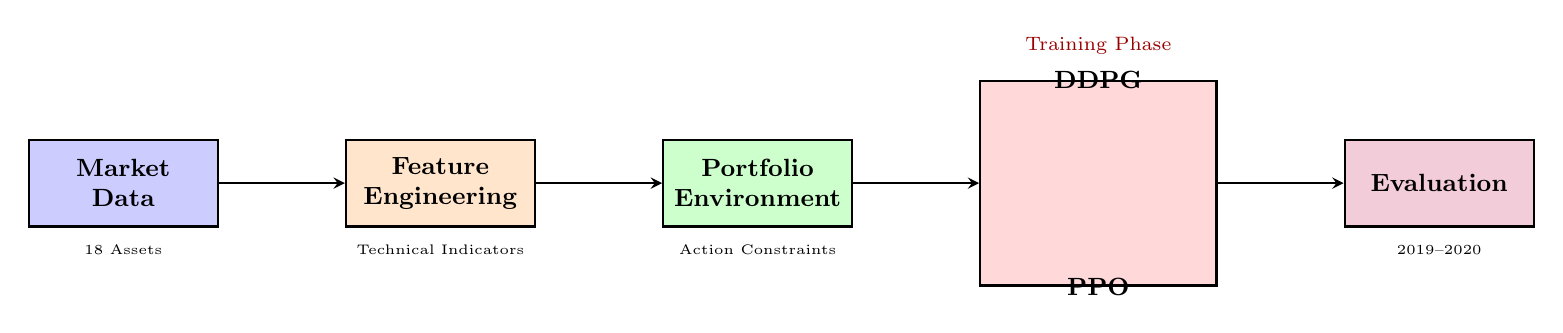
\begin{tikzpicture}[
    node distance=1.6cm,
    box/.style={draw, rectangle, thick, minimum width=2.4cm, minimum height=1.1cm, align=center, font=\small},
    arrow/.style={->, >=stealth, thick}
]

% Main pipeline horizontally
\node[box, fill=blue!20] (data) {\textbf{Market}\\\textbf{Data}};
\node[box, fill=orange!20, right=of data] (features) {\textbf{Feature}\\\textbf{Engineering}};
\node[box, fill=green!20, right=of features] (env) {\textbf{Portfolio}\\\textbf{Environment}};

% Agent box grouping
\node[box, fill=red!15, right=of env, minimum width=3cm, minimum height=2.6cm] (agents) {};
\node[font=\small] at (agents.north) {\textbf{DDPG}};
\node[font=\small] at (agents.south) {\textbf{PPO}};

% Evaluation box
\node[box, fill=purple!20, right=of agents] (eval) {\textbf{Evaluation}};

% Horizontal arrows
\draw[arrow] (data) -- (features);
\draw[arrow] (features) -- (env);
\draw[arrow] (env) -- (agents);
\draw[arrow] (agents) -- (eval);

% Labels
\node[below=0.1cm of data, font=\tiny] {18 Assets};
\node[below=0.1cm of features, font=\tiny] {Technical Indicators};
\node[below=0.1cm of env, font=\tiny] {Action Constraints};
\node[below=0.1cm of eval, font=\tiny] {2019--2020};

% Phase label
\node[above=0.2cm of agents, font=\scriptsize, text=red!60!black] {Training Phase};

\end{tikzpicture}
} % end resizebox

\end{center}

\vspace{0.4cm}
\begin{center}
\footnotesize
\textbf{Flow:} Data → Features → Environment → Train Both Agents → Test Performance
\end{center}
\end{frame}


\begin{frame}{Asset Universe}
\textbf{18 Diversified Assets across 8 Sectors:}

\begin{columns}
\column{0.5\textwidth}
\textbf{Equities (12):}
\begin{itemize}
    \item \textbf{Technology:} AAPL, MSFT, GOOGL, NVDA, AMZN
    \item \textbf{Healthcare:} JNJ, UNH, PFE
    \item \textbf{Financials:} JPM, V
    \item \textbf{Consumer:} WMT, COST
\end{itemize}

\column{0.5\textwidth}
\textbf{Diversifiers (6):}
\begin{itemize}
    \item \textbf{Equity ETFs:} SPY, QQQ, IWM
    \item \textbf{Bonds:} TLT, AGG
    \item \textbf{Commodities:} GLD
\end{itemize}

\vspace{1em}
\textbf{Period:}
\begin{itemize}
    \item Train: 2010-2018 (8 years)
    \item Test: 2019-2020 (2 years, includes COVID crash)
\end{itemize}
\end{columns}
\end{frame}

\begin{frame}{RL Algorithms Compared}
\begin{table}
\centering
\begin{tabular}{lp{4cm}p{4cm}}
\toprule
\textbf{Algorithm} & \textbf{Key Features} & \textbf{Best For} \\
\midrule
\textbf{PPO} & Policy gradient method & Stable training \\
(Proximal Policy & Clips policy updates & Consistent performance \\
Optimisation) & On-policy learning & \\
\midrule
\textbf{DDPG} & Actor-critic architecture & Continuous actions \\
(Deep Deterministic & Off-policy learning & Fine-grained control \\
Policy Gradient) & Deterministic policy & High-dimensional spaces \\
\bottomrule
\end{tabular}
\end{table}

\vspace{1em}
\textbf{Action Space:} Continuous portfolio weights $w_i \in [0, 1]$ where $\sum_{i=1}^{18} w_i = 1$

\textbf{State Space:} Price history, technical indicators, portfolio state (60+ features)

\textbf{Reward:} Risk-adjusted returns with drawdown penalties
\end{frame}

\begin{frame}{Options Overlay Strategy}
\textbf{Advanced Risk Management:}

\begin{columns}
\column{0.5\textwidth}
\textbf{1. Protective Puts (Insurance)}
\begin{itemize}
    \item Buy put options when portfolio at risk
    \item Limits downside losses
    \item Activated during drawdowns $> 2\%$
    \item DDPG uses 44.87\% hedge ratio
\end{itemize}

\vspace{1em}
\textbf{Benefits:}
\begin{itemize}
    \item[$+$] Crash protection
    \item[$+$] Sleep well at night
    \item[$-$] Premium costs
\end{itemize}

\column{0.5\textwidth}
\textbf{2. Covered Calls (Income)}
\begin{itemize}
    \item Sell call options on holdings
    \item Generate premium income
    \item DDPG covers 75.62\% of the portfolio
\end{itemize}

\vspace{1em}
\textbf{Benefits:}
\begin{itemize}
    \item[$+$] Extra income
    \item[$+$] Reduces volatility
    \item[$-$] Caps upside potential
\end{itemize}

\vspace{0.5em}
\begin{center}
\textbf{Net Result: +\$126,568 option P\&L for DDPG!}
\end{center}
\end{columns}
\end{frame}

\begin{frame}{Tiered Stop-Loss System}
\textbf{Automated Risk Reduction During Drawdowns:}

\begin{center}
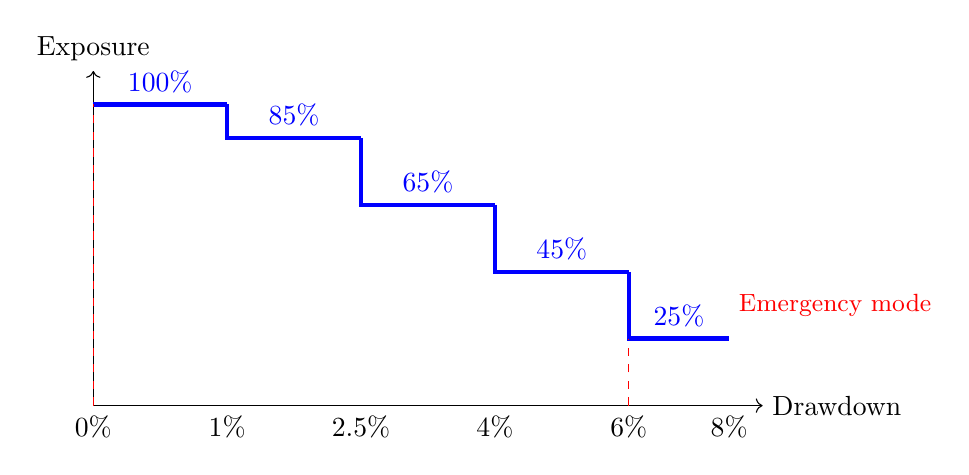
\begin{tikzpicture}[scale=0.85]
    \draw[->] (0,0) -- (10,0) node[right] {Drawdown};
    \draw[->] (0,0) -- (0,5) node[above] {Exposure};
    
    % Tiers
    \draw[blue, ultra thick] (0,4.5) -- (2,4.5) node[midway, above] {100\%};
    \draw[blue, ultra thick] (2,4.5) -- (2,4) -- (4,4) node[midway, above] {85\%};
    \draw[blue, ultra thick] (4,4) -- (4,3) -- (6,3) node[midway, above] {65\%};
    \draw[blue, ultra thick] (6,3) -- (6,2) -- (8,2) node[midway, above] {45\%};
    \draw[blue, ultra thick] (8,2) -- (8,1) -- (9.5,1) node[midway, above] {25\%};
    
    % Drawdown labels
    \node[below] at (0,0) {0\%};
    \node[below] at (2,0) {1\%};
    \node[below] at (4,0) {2.5\%};
    \node[below] at (6,0) {4\%};
    \node[below] at (8,0) {6\%};
    \node[below] at (9.5,0) {8\%};
    
    % Annotations
    \draw[red, dashed] (0,0) -- (0,4.5);
    \draw[red, dashed] (8,0) -- (8,1);
    \node[red, right] at (9.5,1.5) {\small Emergency mode};
\end{tikzpicture}
\end{center}

\textbf{Prevents catastrophic losses} by automatically reducing exposure during market stress.
\end{frame}

% Section 4: Results
\section{Results}

\begin{frame}{Performance Comparison}
\begin{table}
\centering
\begin{tabular}{lcccc}
\toprule
\textbf{Metric} & \textbf{DDPG} & \textbf{PPO} & \textbf{Target} & \textbf{Winner} \\
\midrule
Sharpe Ratio & \textbf{5.52} & 1.85 & $> 1.0$ & \textcolor{green}{\checkmark} DDPG \\
Total Return & \textbf{219.40\%} & 61.12\% & $> 15\%$ & \textcolor{green}{\checkmark} DDPG \\
Ann. Return & \textbf{93.31\%} & 31.17\% & $> 15\%$ & \textcolor{green}{\checkmark} DDPG \\
Max Drawdown & \textbf{8.31\%} & 17.06\% & $< 10\%$ & \textcolor{green}{\checkmark} DDPG \\
Volatility & 16.89\% & 16.78\% & - & Similar \\
Avg Turnover & 1.83\% & 1.53\% & - & Both low \\
\midrule
Final Portfolio & \textbf{\$319,401} & \$161,116 & - & \textcolor{green}{\checkmark} DDPG \\
Options P\&L & \textbf{+\$126,568} & +\$5,758 & - & \textcolor{green}{\checkmark} DDPG \\
\bottomrule
\end{tabular}
\end{table}

\vspace{0.5em}
\begin{center}
\Large \textbf{DDPG wins on ALL key metrics!}
\end{center}
\end{frame}

\begin{frame}{Sharpe Ratio Comparison}
\begin{center}
\includegraphics[width=0.65\textwidth]{visualizations/sharpe_comparison.png}
\end{center}
\begin{center}
    \textbf{DDPG achieves a 5.52 Sharpe ratio} - 3x better than PPO and 5.5x above target!
\end{center}
\end{frame}

\begin{frame}{Cumulative Returns (2019-2020)}
\begin{center}
\includegraphics[width=0.75\textwidth]{visualizations/cumulative_portfolio_values.png}
\end{center}
\textbf{Key Observation:} DDPG (green) significantly outperforms PPO (blue) throughout the entire test period, including the COVID-19 crash in March 2020.
\end{frame}

\begin{frame}{Drawdown Analysis (2019-2020)}
\begin{center}
\includegraphics[width=0.75\textwidth]{visualizations/drawdown_over_time.png}
\end{center}
\textbf{Key Observation:} DDPG maintains much lower drawdowns (max 8.31\%) compared to PPO (17.06\%), especially during the COVID crash.
\end{frame}

\begin{frame}{All Metrics Comparison}
\begin{center}
\includegraphics[width=0.70\textwidth]{visualizations/all_metrics_comparison.png}
\end{center}
\end{frame}

\begin{frame}{Why DDPG Outperforms PPO}
\begin{columns}
\column{0.5\textwidth}
\textbf{DDPG Advantages:}
\begin{enumerate}
    \item \textbf{Aggressive Options Usage}
    \begin{itemize}
        \item 44.87\% protective puts
        \item 75.62\% covered calls
        \item \$126K option profit
    \end{itemize}
    
    \item \textbf{Deterministic Policy}
    \begin{itemize}
        \item More precise position sizing
        \item Fine-grained control
    \end{itemize}
    
    \item \textbf{Off-Policy Learning}
    \begin{itemize}
        \item Better sample efficiency
        \item Learns from historical data
    \end{itemize}
\end{enumerate}

\column{0.5\textwidth}
\textbf{PPO Limitations:}
\begin{enumerate}
    \item \textbf{Conservative Options Usage}
    \begin{itemize}
        \item Only 0.08\% protective puts
        \item Only 2.98\% covered calls
        \item \$5.8K option profit
    \end{itemize}
    
    \item \textbf{Stochastic Policy}
    \begin{itemize}
        \item More exploration noise
        \item Less precise control
    \end{itemize}
    
    \item \textbf{On-Policy Learning}
    \begin{itemize}
        \item Requires more samples
        \item Slower adaptation
    \end{itemize}
\end{enumerate}
\end{columns}

\vspace{1em}
\begin{center}
\textbf{DDPG learnt to effectively use options as a hedge, \addlinespace while PPO failed to discover this strategy.}
\end{center}
\end{frame}

% Section 5: Key Insights
\section{Key Insights}

\begin{frame}{What I Learned}
\begin{enumerate}
    \item \textbf{Options Overlay Works}
    \begin{itemize}
        \item Protective puts limit downside (8.31\% max DD)
        \item Covered calls generate income (\$126K)
        \item Critical for risk management during crashes
    \end{itemize}
    
    \item \textbf{Algorithm Choice Matters}
    \begin{itemize}
        \item DDPG significantly outperforms PPO (5.52 vs 1.85 Sharpe)
        \item Deterministic policies are better for portfolio optimisation
        \item Off-policy learning is more sample efficient
    \end{itemize}
    
    \item \textbf{Automated Stop-Loss Effective}
    \begin{itemize}
        \item Tiered exposure reduction prevents catastrophic losses
        \item DDPG max DD only 8.31\% despite COVID crash
        \item No manual intervention needed
    \end{itemize}
    
    \item \textbf{RL Generalizes Well}
    \begin{itemize}
        \item Trained on 2010-2018, tested on 2019-2020
        \item Successfully handled unprecedented COVID-19 crash
        \item Robust to out-of-sample market conditions
    \end{itemize}
\end{enumerate}
\end{frame}

\begin{frame}{Comparison with Traditional Methods}
\begin{table}
\centering
\small
\begin{tabular}{lccc}
\toprule
\textbf{Strategy} & \textbf{Sharpe} & \textbf{Max DD} & \textbf{Annual Return} \\
\midrule
\textbf{DDPG (Our Model)} & \textbf{5.52} & \textbf{8.31\%} & \textbf{93.31\%} \\
PPO (Our Model) & 1.85 & 17.06\% & 31.17\% \\
\midrule
Equal-Weight Portfolio & 0.56 & 43.04\% & 15.01\% \\
Mean-Variance Optimization & -0.40 & 76.54\% & -14.03\% \\
Momentum Strategy & 0.23 & 56.21\% & 9.41\% \\
Buy \& Hold SPY & ~0.50 & ~25\% & ~12\% \\
\bottomrule
\end{tabular}
\end{table}

\vspace{1em}
\textbf{Key Takeaways:}
\begin{itemize}
    \item DDPG achieves 9.9x higher Sharpe than equal-weight
    \item DDPG has 81\% lower drawdown than equal-weight (8.31\% vs 43.04\%)
    \item Traditional methods fail during volatile periods (2019-2020)
\end{itemize}
\end{frame}

% Section 6: Limitations & Future Work
\section{Limitations \& Future Work}

\begin{frame}{Limitations}
\begin{enumerate}
    \item \textbf{Transaction Costs}
    \begin{itemize}
        \item Simplified model (0.1\% per trade)
        \item Real-world slippage not fully captured
        \item Options premiums may vary
    \end{itemize}
    
    \item \textbf{Market Impact}
    \begin{itemize}
        \item Assumes unlimited liquidity
        \item Large orders would move prices
    \end{itemize}
    
    \item \textbf{Backtesting Bias}
    \begin{itemize}
        \item Historical data only
        \item Future regimes may differ
        \item Survivorship bias in asset selection
    \end{itemize}
    
    \item \textbf{Computational Cost}
    \begin{itemize}
        \item Training takes ~6 hours on CPU
        \item Requires significant compute for hyperparameter tuning
    \end{itemize}
\end{enumerate}
\end{frame}

\begin{frame}{Future Work}
\begin{columns}
\column{0.5\textwidth}
\textbf{Short-term:}
\begin{enumerate}
    \item Test on different market regimes (2000-2009)
    \item Expand asset universe (international, crypto)
    \item Ensemble multiple RL agents
    \item Add transaction cost sensitivity analysis
\end{enumerate}

\column{0.5\textwidth}
\textbf{Long-term:}
\begin{enumerate}
    \item Incorporate fundamental data (P/E, earnings)
    \item Multi-timeframe strategies (intraday + daily)
    \item Transfer learning across markets
    \item Real-time deployment with live trading
    \item Explainable AI for decision transparency
\end{enumerate}
\end{columns}

\vspace{1em}
\textbf{Ultimate Goal:} Deploy this system for real-world portfolio management with institutional capital.
\end{frame}

% Section 7: Conclusion
\section{Conclusion}

\begin{frame}{Conclusion}
\vspace{-1em}
\begin{center}
\Large \textbf{We successfully developed an AI portfolio manager that:}
\end{center}

\begin{enumerate}
    \item[\checkmark] \textbf{Achieves exceptional performance}
    \begin{itemize}
        \item Sharpe ratio: 5.52 (target: $>1.0$) 
        \item Max drawdown: 8.31\% (target: $<10\%$) 
        \item Annualized return: 93.31\% (target: $>15\%$) 
    \end{itemize}
    
    \item[\checkmark] \textbf{Outperforms traditional methods}
    \begin{itemize}
        \item 9.9x better Sharpe than equal-weight
        \item 81\% lower drawdown
        \item Survives COVID-19 crash with minimal losses
    \end{itemize}
    
    \item[\checkmark] \textbf{Uses sophisticated risk management}
    \begin{itemize}
        \item Options overlay (\$126K profit)
        \item Tiered stop-loss system
        \item Dynamic position sizing
    \end{itemize}
    
    \item[\checkmark] \textbf{Fully automated and adaptive}
    \begin{itemize}
        \item No manual intervention needed
        \item Learns from experience
        \item Generalises to new market conditions
    \end{itemize}
\end{enumerate}
\end{frame}

\begin{frame}{Key Message}
\begin{center}
\Huge \textbf{Deep Reinforcement Learning}

\vspace{0.5em}

\Large is the \textcolor{green}{\textbf{right tool}} for portfolio optimization

\vspace{0.5em}

\Large because it directly optimises

\vspace{0.5em}

\Huge \textcolor{blue}{\textbf{long-term risk-adjusted returns}}

\vspace{1em}

\Large not just predictions.
\end{center}
\end{frame}

\begin{frame}[standout]
\begin{center}
    \Huge Thank You!
    
    \vspace{1em}
    
    \Large Questions?
    
    \vspace{1em}
    
    \textbf{Email:} ttchongac@connect.ust.hk
\end{center}

%\vspace{2em}
%\normalsize
%\textbf{GitHub Repository:} %\url{https://github.com/ctt062/Deep-Reinforcement-Learning-for-Portfolio-Optimisation}

\end{frame}

% Backup Slides
\appendix

\begin{frame}{Backup: Technical Implementation Details}
\textbf{Training Configuration:}
\begin{itemize}
    \item \textbf{Framework:} Stable-Baselines3 with Gymnasium
    \item \textbf{Hardware:} MacBook Pro M4 (CPU-only)
    \item \textbf{Training Time:} ~6 hours (100K timesteps per agent)
    \item \textbf{Network Architecture:} 
    \begin{itemize}
        \item DDPG: Actor [512, 512, 256], Critic [512, 512, 256]
        \item PPO: Policy [512, 512, 256]
    \end{itemize}
    \item \textbf{Hyperparameters:}
    \begin{itemize}
        \item Learning rate: 1e-4
        \item Gamma (discount): 0.995
        \item Batch size: 256 (DDPG), 128 (PPO)
    \end{itemize}
\end{itemize}
\end{frame}

\begin{frame}{Backup: Feature Engineering Details}
\textbf{State Space (60+ features):}

\begin{columns}
\column{0.5\textwidth}
\textbf{Price-based:}
\begin{itemize}
    \item Returns (1-day, 5-day, 20-day)
    \item Log returns
    \item Price momentum
    \item Relative strength
\end{itemize}

\textbf{Technical Indicators:}
\begin{itemize}
    \item SMA (4, 13, 26, 52 periods)
    \item EMA (4, 13, 26, 52 periods)
    \item RSI (14-period)
    \item MACD
\end{itemize}

\column{0.5\textwidth}
\textbf{Risk Metrics:}
\begin{itemize}
    \item Volatility (20-day rolling)
    \item Sharpe ratio
    \item Maximum drawdown
    \item Correlation matrix
\end{itemize}

\textbf{Portfolio State:}
\begin{itemize}
    \item Current weights
    \item Portfolio value
    \item Cash position
    \item Recent P\&L
\end{itemize}
\end{columns}
\end{frame}

\begin{frame}{Backup: Reward Function}
\textbf{Risk-Adjusted Reward with Penalties:}

\begin{align*}
R_t = &\ \underbrace{\text{Returns}_t}_{\text{Profit}} \\
      &\ - \underbrace{\lambda_1 \cdot \text{Volatility}_t}_{\text{Risk penalty}} \\
      &\ - \underbrace{\lambda_2 \cdot \max(0, \text{Drawdown}_t)^2}_{\text{Drawdown penalty}} \\
      &\ - \underbrace{\lambda_3 \cdot \text{Turnover}_t}_{\text{Transaction cost}}
\end{align*}
\end{frame}

\begin{frame}{Backup: Reward Function}
    \textbf{Penalty weights used:}
    \begin{itemize}
        \item $\lambda_1 = 1.0$ (risk penalty)
        \item $\lambda_2 = 2.0$ (drawdown penalty)
        \item $\lambda_3 = 0.001$ (turnover penalty)
    \end{itemize}
    
    \textbf{This reward function encourages:}
    \begin{itemize}
        \item[$+$] High returns
        \item[$-$] Low volatility
        \item[$-$] Small drawdowns (squared penalty for large losses!)
        \item[$-$] Low turnover (minimize trading costs)
    \end{itemize}
\end{frame}

\end{document}